\documentclass[12pt]{exam}

\newcommand{\course}{MTH 234 Summer 2021}
\newcommand{\qdate}{13.2 and 13.3} %PUT DATE HERE
\newcommand{\quiz}{Group Work} 

    \usepackage[top=1in, bottom=1in, left=.45in, right=.45in]{geometry}
    \usepackage{amsmath,amsthm,amssymb,amstext}
    \usepackage{enumerate,enumitem}
    \usepackage{tikz,float,graphicx}
    \usepackage{microtype}
    \usepackage{bm,tikz}
        \usetikzlibrary{calc}
    \usepackage{multicol}
    \usepackage{nicematrix}
    \usepackage{cleveref}
    \usepackage[framemethod=tikz]{mdframed}
    
    %\newcommand{\course}{MTH 234 Summer 2021}
    %\newcommand{\qdate}{Equations of lines and planes} %PUT DATE HERE
    %\newcommand{\quiz}{Group Work} 
    
    \newcommand{\R}{\mathbb{R}}
    
    \newcommand{\ba}{\bm{a}}
    \newcommand{\bb}{\bm{b}}
    \newcommand{\bc}{\bm{c}}
    \newcommand{\bi}{\bm{i}}
    \newcommand{\bj}{\bm{j}}
    \newcommand{\bk}{\bm{k}}
    \newcommand{\br}{\bm{r}}
    \newcommand{\bv}{\bm{v}}
    \newcommand{\gen}[1]{\left\langle #1 \right\rangle}

\newtheorem*{theorem}{Theorem}
\surroundwithmdframed[]{theorem}

\theoremstyle{definition}
    \newtheorem*{definition}{Definition}
    \surroundwithmdframed[]{definition}
    \newtheorem*{info}{Useful Information}
    \surroundwithmdframed[]{info}
\theoremstyle{remark}
    \newtheorem*{remark}{Remark}
    \surroundwithmdframed[]{remark}
    

%%%%%%%%%%%%%%%%%%%%%%%
% HEADER AND FOOTER
%%%%%%%%%%%%%%%%%%%%%%%
\pagestyle{headandfoot}
\firstpageheadrule
\runningheadrule
\firstpageheader{\course}{\quiz}{\qdate}
\runningheader{\course}{\quiz}{\qdate}
\runningfooter{}{}{}


\usepackage{color}
\shadedsolutions
\definecolor{SolutionColor}{rgb}{0.8,0.9,1}

\usepackage{pgfplots}
    \pgfplotsset{every axis/.append style={
                    axis x line=middle,    % put the x axis in the middle
                    axis y line=middle,    % put the y axis in the middle
                    axis line style={<->}, % arrows on the axis
                    xlabel={$x$},          % default put x on x-axis
                    ylabel={$y$},          % default put y on y-axis
                    grid=both,
                    %xtick={-4,...,-1,1,...,3},
                    %ytick={-1,1,}
    }}
    \pgfplotsset{compat=1.17}

\newcommand{\bif}{\quad\iff\quad}
\newcommand{\bu}{\bm{u}}
\newcommand{\bT}{\text{\textbf{T}}}
\newcommand{\bN}{\text{\textbf{N}}}
\newcommand{\bB}{\text{\textbf{B}}}
\newcommand{\LR}[1]{\left(#1\right)}

\printanswers
%\noprintanswers

\begin{document}

\section*{13.2  Derivatives and Integrals of Vector Functions}

\begin{questions}

\question For each of the following 
    \begin{enumerate}[label=$(\roman*)$]
        \item Sketch the following curves in the \(xy\)-plane
        \item Find \(\br'(t)\)
        \item Sketch the tangent vector \(\br'(t)\) for the given value of \(t\)
    \end{enumerate}

~

    \begin{parts}
        \part \(\br(t)=\gen{t^2,t^3}\) with \(t=-1\)
        
\ifprintanswers
        \begin{solution}
            At \(t=-1\) the curve \(\br(t)\) passes through \(\br(-1)=(1,-1)\).
            Since \(\br'(t) = \gen{2t,3t^2}\), the tangent vector at that point is given by \(\br'(-1)=\gen{-2,3}\). 
            
            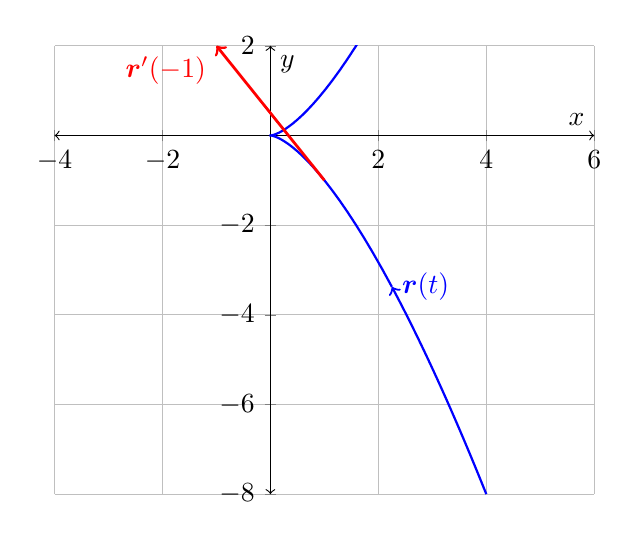
\begin{tikzpicture}
                \begin{axis}[xmin=-4,xmax=6,ymin=-8,ymax=2]
                    \addplot[->,variable=t,blue,thick,mark=none,domain=-1.5:1.5,samples=50] ({(\t)^2},{(\t)^3});
                    \addplot[->,variable=t,blue,thick,mark=none,domain=-2:-1.5,samples=50] ({(\t)^2},{(\t)^3}) node[anchor=west] {$\br(t)$};
                    \addplot[->,variable=t,red,very thick,mark=none,domain=0:1,line width=1pt] ({1-2*\t},{-1+3*\t}) node[anchor=north east] {$\br'(-1)$};
                \end{axis}
            \end{tikzpicture}
        \end{solution}
    \else
        \vfill
    \fi

        \part \(\br(t)=\gen{t-2,t^2+1}\) with \(t=1\)
        
    \ifprintanswers
        \begin{solution}
            At \(t=1\) the curve passes through \(\br(1)=\gen{-1,2}\). Also \(\br'(t)=\gen{1,2t}\) and \(\br'(1)=\gen{1,2}\).
            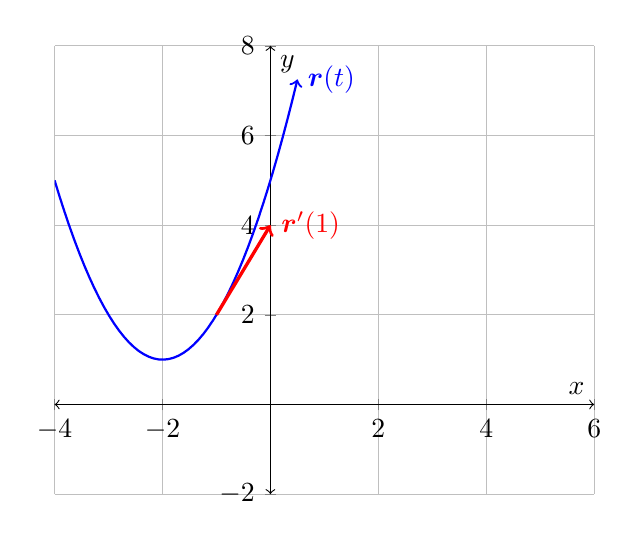
\begin{tikzpicture}
                \begin{axis}[xmin=-4,xmax=6,ymin=-2,ymax=8]
                    \addplot[->,variable=t,blue,thick,mark=none,domain=-2:2.5,samples=50] ({\t-2},{(\t)^2+1}) node[anchor=west] {$\br(t)$};
                    \addplot[->,variable=t,red,very thick,mark=none,domain=0:1] ({-1+t},{2+2*\t}) node[anchor=west] {$\br'(1)$};
                \end{axis}
            \end{tikzpicture}
        \end{solution}
    \else
        \vfill
    \fi
    \end{parts}

    \newpage

\question Find \(\br'(t)\) given \(\br(t)=\gen{t\sin(t),t^2,\cos(2t)}\)
    
\ifprintanswers
        \begin{solution}
            \begin{align*}
                \br'(t) & = \gen{\frac{d}{dt}(t\sin(t)),\frac{d}{dt}(t^2),\frac{d}{dt}(\cos(2t))}\\
                    & = \gen{(1)\sin(t)+t\cos(t),2t,-2\sin(2t)}\\
                    \br'(t) & = \gen{\sin(t)+t\cos(t),2t,-2\sin(2t)}
            \end{align*}
        \end{solution}
    \else
        \vfill
    \fi

\question Find parametric equations for the tangent line to the curve \(\bv(t)=\gen{1+2\sqrt{t},t^3-t,t^3+t}\) at the point \((3,0,2)\)
    
\ifprintanswers
        \begin{solution}
            To find the value of \(t\) that makes \(\bv(t)=(3,0,2)\) set the components equal:
            \[
                1 + 2\sqrt{t}=3 \quad\Rightarrow\quad t=1
            \]
            From \(\bv'(t)=\gen{\frac{1}{\sqrt{t}},3t^2-1,3t^2+1}\) and \(\bv'(1)=\gen{1,2,4}\), the tangent line is represented by 
            \begin{align*}
                \bu(t) & = \gen{3,0,2}+t\gen{1,2,4}\\
                    & = \gen{3+t,2t,2+4t}.
            \end{align*}
            In particular 
            \begin{gather*}
                x(t) = 3+t\\
                y(t) = 2t\\
                z(t) = 2+4t
            \end{gather*}
        \begin{center}
            \includegraphics[width=.5\textwidth]{hardthing.pdf}

            In the above \(\bv(t)\) is shown in green and the the line we found is shown in blue.
        \end{center}
        \end{solution}
    \else
        \vfill
    \fi


\newpage 

\question Evaluate the given integrals
    \begin{parts}
        \part 
            \[
                \int_{0}^{2} \left( t\bi-t^2\bj+3t^5\bk \right) ~dt
            \]
        
\ifprintanswers
        \begin{solution}
            \begin{align*}
                \int_{0}^{2} \left( t\bi-t^2\bj+3t^5\bk \right) ~dt & = \LR{\int_{0}^{2}t~dt}\bi-\LR{\int_{0}^{2}t^2~dt}\bj+\LR{\int_{0}^{2}3t^5~dt}\bk\\
                    & = \LR{\frac{1}{2}t^2\bigg|_{0}^{2}}\bi-\LR{\frac{1}{3}t^3\bigg|_{0}^{2}}\bj+\LR{\frac{1}{2}t^{6}\bigg|_{0}^{2}}\bk\\
                    & = 2\bi-\frac{8}{3}\bj+32\bk
            \end{align*}
        \end{solution}
    \else
        \vfill
    \fi

        \part 
            \[
                \int_{0}^{1}\left( \dfrac{4}{1+t^2}\bj+\dfrac{2t}{1+t^2}\bk \right) ~dt
            \]

\ifprintanswers
        \begin{solution}
        \begin{align*}
            \int_{0}^{1}\left( \dfrac{4}{1+t^2}\bj+\dfrac{2t}{1+t^2}\bk \right) ~dt
                & = \LR{4\tan^{-1}(t)\bigg|_{0}^{1}}\bj
                    + \LR{\ln(1+t^2)\bigg|_{0}^{1}}\bk\\
                & = 4\cdot\frac{\pi}{4}\bj+\ln(2)\bk\\
                & = \pi\bj+\ln(2)\bk
        \end{align*}
        \end{solution}
    \else
        \vfill
    \fi 
    \end{parts}

%\question The curves 
%\[
%    \br_1(t) = \gen{t,t^2,t^3} \quad\text{and}\quad \br_2(t)=\gen{\sin(t),\sin(2t),t}
%\]
%intersect at the point \((0,0,0)\). Find the angle of intersection

\newpage

\section*{13.3 Arc Length and Curvature}

\begin{align*}
    \text{Unit tangent vector}\quad & \bT(t) = \dfrac{\br'(t)}{|\br'(t)|} \\
                \text{Unit normal vector}\quad & \bN(t) = \dfrac{\bT(t)}{|\bT'(t)|} \\
                \text{Binormal vector}\quad & \bB(t) = \bT(t)\times \bN(t)\\
                \text{Curvature}\quad & \kappa(t)=\left|\dfrac{d\bT}{ds}\right| = \dfrac{|\bT'(t)|}{|\br'(t)|} = \dfrac{|\br'(t)\times \br''(t)|}{|\br'(t)|^3}
\end{align*}

\question Find the unit tangent vector \(\bm{T}(\pi/4)\) to the curve \(\gen{\sin^2(t),\cos^2(t),\tan^2(t)}\).
    
\ifprintanswers
        \begin{solution}
            \begin{align*}
                \br'(t) & = \gen{2\sin(t)\cos(t),-2\cos(t)\sin(t),2\tan(t)\sec^2(t)}\\
                \br'(\pi/4) & = \gen{1,-1,4}\\
                |\br'(\pi/4)| & = \sqrt{1+1+16}\\
                \bT(\pi/4) & = \gen{\frac{1}{\sqrt{18}},-\frac{1}{\sqrt{18}},\frac{4}{\sqrt{18}}}
            \end{align*}
        \end{solution}
    \else
        \vfill
    \fi


\question Suppose you are at the point \((0,0,0)\) and move \(2\) units in the positive direction along the curve \(\br(t)=\gen{t^2,t^3,t^4}\). What point did you end up at? (Your answer may be messy, if so do not try to simplify.)
\ifprintanswers
        \begin{solution}
            %The curve \(\br(t)\) passes through \((0,0,0)\) when \(t=0\). Let \(P\) be the point you arrive at after moving 2 units in the positive direction, and let \(s\) be the value for which \(\br(s)%=P\).%
%
%            %Then 
%            %\begin{align*}
%            %    2 & = \int_{0}^{s}|\br'(t)|dt\\
%            %        & = \int_{0}^{s}|\gen{2t,3t^2,4t^3}|dt\\
            %        & = \int_{0}^{s}\sqrt{4t^2+9t^4+16t^6}\\
            %\end{align*}

            
        \end{solution}
    \else
        \vfill
    \fi    


    \question Find the length of the curve \(\br(t)=\bi+t^2\bj+t^3\bk\) with \(0\le t\le 1\). Then find the unit tangent vector \(\bm{T}(t)\) and unit normal vector \(\bm{N}(t)\).
    

        \ifprintanswers
        \begin{solution}

        \end{solution}
    \else
        \vfill
    \fi     

\end{questions}

\end{document}
